\documentclass[12pt]{article}

% Language
\usepackage[english]{babel} % or [english] depending on your thesis language
%\usepackage[utf8]{inputenc}
\usepackage[T1]{fontenc}

% Page layout
\usepackage[a4paper, top=2cm, bottom=2cm, left=2.5cm, right=2.5cm]{geometry}

% Essential packages
\usepackage{graphicx}
\usepackage{amsmath}
\usepackage{enumitem}
\usepackage[colorlinks=true, allcolors=blue]{hyperref}
\usepackage{setspace}
\usepackage{csquotes}
\usepackage{newtxtext,newtxmath}  % Times-like text and math
\usepackage[backend=biber, style=numeric]{biblatex}
\usepackage{float}
\addbibresource{bibliography.bib}
\setstretch{1.2} % Optional, for slight line spacing

% Font: use default Latin Modern – nothing else needed

% No page numbers on title page
\pagestyle{plain}

\begin{document}

% Include title
%!TEX root = ../../main.tex

\begin{titlepage}
\thispagestyle{empty} % No page number

% Ensure serif font — default is Latin Modern
\rmfamily

\vspace*{-1.5cm}

\begin{figure}[ht]
\centering
\begin{minipage}{0.45\textwidth}
    \centering
    
\includegraphics[height=30mm]{files/RFT_Logo}
\end{minipage}%
\hfill
\begin{minipage}{0.45\textwidth}
    \centering
    
\includegraphics[height=30mm]{files/TU_Logo_lang_RGB_rot}
\end{minipage}
\end{figure}

\vspace{2.5cm}

\begin{center}
    Technische Universität Berlin\\
    Fakultät V für Maschinenbau und Verkehrssysteme

    \vspace{2cm}

    Bachelor's Thesis

    \vspace{1.5cm}

    \begin{spacing}{1.3}
    \textbf{\LARGE
        Implementation of an AI-Algorithm for cloud\\
        detection on an embedded system tensor\\
        processing unit\\}
    \end{spacing}

    \vspace{2cm}

    Author:\\
    Andrei Zharski

    \vspace{1cm}

    \today
\end{center}

\vfill

\noindent
\begin{minipage}[t]{0.48\textwidth}
    Supervisor:\\
    Prof. Dr.-Ing Enrico Stoll\\
    Lehrstuhl für Raumfahrttechnik\\
    Technische Universität Berlin
\end{minipage}%
\hfill
\begin{minipage}[t]{0.48\textwidth}
    \raggedleft
    Second supervisor:\\
    M.Sc. Alexander Balke\\
\end{minipage}


\end{titlepage}


% the second page
%\thispagestyle{empty}
%\vspace*{\fill}
%\begin{minipage}{15.0cm}
%    Zharski, Andrei:\\
%    \emph{Implementation of an AI-Algorithm for cloud
%        detection on an embedded system tensor
%        processing unit\\}
%    Bachelor Thesos, Technische Universität Berlin, 2025.
%\end{minipage}
%\newpage
%!TEX root = ../../main.tex

\chapter*{Selbständigkeitserklärung gemäß § 60 Abs. 8 AllgStuPO}


Hiermit erkläre ich, dass ich die vorliegende Arbeit selbstständig und eigenhändig sowie ohne unerlaubte Hilfe und ausschließlich unter Verwendung der aufgeführten Quellen und Hilfsmittel angefertigt habe.  
Die selbstständige und eigenhändige Anfertigung versichere ich an Eides statt.


\vspace{3cm}

\noindent\begin{tabular}{ll}
    \makebox[65mm]{\hrulefill} & \makebox[65mm]{\hrulefill} \\
    Datum, Ort & Unterschrift der/des Studierenden
\end{tabular}

\chapter*{Agreement on utilization rights}
{

\setlength{\parindent}{0pt}
\setlength{\parskip}{1em}

According to § 60 of the AllgStuPO, students of the TU Berlin must complete a final thesis during their studies. The totality of the achievements associated with a final thesis are based not only on the written documentation and the commitment of the student, but also on the supervisory effort of the department, including the preparation of the assignment, the specific requirements, guidance of the students, help and advice in organizational, technical and scientific terms. Therefore, the student is the sole author of the written work, but not the sole author of the entirety of the services associated with a thesis.


By supervising the student, the Technische Universität Berlin, represented by the Chair of Astronautics, becomes co-author of the entirety of the achievements and the associated results according to § 8 section 1 of the German Copyright Act (Urheberrechtsgesetz).


For non-profit use in teaching and research, the Chair may use the results of the present work. As co-author, the chair is entitled to do so according to § 8 section 2 of the Copyright Act. If the work is written independently in such a way that there is no co-authorship, this right of use is granted by the student according to § 31 section 2 of the Copyright Act. This right of use is unrestricted and includes content of any kind (e.g. documentation, presentations, photos, videos, procedures, drafts, drawings, software including source code and the like) with naming of the author.


Due to the reference to ongoing research projects, publication without explicit permission of the department will not be permitted to the student. This is to be checked and approved by the department in each individual case.


Any commercial use of either site will only occur with the consent of all authors of the present work, with appropriate participation in the earnings.

}
\vspace{3cm}

\noindent\begin{tabular}{ll}
    \makebox[65mm]{\hrulefill} & \makebox[65mm]{\hrulefill} \\
    Date, Place & Signature of the Student
\end{tabular}
%!TEX root = ../main.tex
{

\setlength{\parindent}{0pt}
\setlength{\parskip}{1em}

\section*{Zusammenfassung}
\addcontentsline{toc}{section}{Zusammenfassung}

Die Technische Universität Berlin hat am 01.01.2022 das Projekt AITHER ins Leben gerufen. Im Rahmen dieses Projekts wurde der \textit{OOV-CUBE} Satellit in die Erdumlaufbahn gebracht. An Bord befindet sich die KI-Daten\-ver\-ar\-bei\-tungs\-ein\-heit, auf der rechenintensive und zuverlässige Aufgaben durchgeführt werden sollen. Ziel des Projekts ist die Untersuchung der Strahlungstoleranz verschiedener Onboard-Architekturen unter Welt\-raum\-be\-ding\-un\-gen. Zu diesem Zweck soll ein KI-Modell entwickelt werden, das Rechenoperationen direkt an Bord ausführt. Die Aufgabe zur Wolkenerkennung auf den aufgenommenen Satellitenbildern eignet sich besonders gut dafür. Für die Berechnungen ist der KI-Beschleuniger -- in diesem Fall eine \textit{Tensor Processing Unit} (TPU) auf einem \textit{Google Coral Dev Board} -- zuständig. Die TPU wird die Tensoroperationen des Algorithmus zur Wolkenerkennung direkt im Orbit ausführen.

In dieser Bachelorarbeit wird die Erkennung der Wolken auf den Satellitenbildern mithilfe von \textit{Convolutional Neural Network} (CNN) implementiert. Als Ausgangspunkt werden die \textit{state of the art} Architekturen der bestehenden CNNs zur Wolkenerkennung untersucht, wie sie beispielsweise in den wissenschaftlichen Artikeln \cite{CloudNet2019} und \cite{CloudDet2018} beschrieben sind. Das CNN wird speziell für die Ausführung auf einer eingebetteten Plattform \textit{Google Coral Dev Board} angepasst. Die fertige Lösung soll eine miniaturisierte Onboard-Da\-ten\-ver\-ar\-bei\-tungs\-ein\-heit sein, die auf den aufgenommenen Bildern direkt auf dem Satelliten im Orbit die Wolken erkennen kann.

Es wird ein Datensatz aus der Landsat 8 Mission verwendet. Er umfasst 38 Wolkenbilder, die aus 4 Kanälen bestehen: Rot, Grün, Blau und Nahinfrarot. Um das Modell zu trainieren und zu validieren, wird dieser in Trainings- und Testdaten aufgeteilt. Die Funktionalität des Modells soll überprüft werden und die Performanz auf dem eingebetteten System wird evaluiert. 

In weiteren Schritten sollte die Software auf den sich bereits im Orbit befindenden Satelliten \textit{OOV-CUBE} hochgeladen werden. Mit folgender wissenschaftlicher Mission wird nicht nur die Robustheit der handelsüblichen elektronischen Komponenten gegenüber kosmischen Strahlung untersucht, sondern auch die Möglichkeit geprüft, den Downlink vom Satelliten zur Erde zu entlasten, um die Effizienz von Erdbeobachtungs- und Kommunikationsmissionen zu erhöhen.

\newpage

\section*{Abstract}
\addcontentsline{toc}{section}{Abstract}

The Technical University of Berlin launched the AITHER project on January 1st, 2022. As part of this project the OOV-CUBE satellite was placed into Earth orbit. An onboard AI data processing unit is designed to perform computationally intensive and reliable tasks. The goal of the project is to study the radiation tolerance of different onboard architectures under space conditions. For this purpose, an AI model is being developed to perform calculations directly onboard. Cloud detection in satellite images is particularly well suited for this task. These computations are carried out by a dedicated AI hardware accelerator --- a Tensor Processing Unit (TPU) embedded on a Google Coral Dev Board. The TPU will execute the tensor operations of the cloud detection algorithm directly in orbit.

In this bachelor's thesis, the detection of clouds in satellite images is implemented using Convolutional Neural Network (CNN). The thesis begins by reviewing state-of-the-art CNN architectures for cloud detection, as described in scientific articles \cite{CloudNet2019} and \cite{CloudDet2018}. The CNN is specifically adapted to run on the embedded Google Coral Dev Board. The final solution will be a miniaturized data processing unit capable of detecting clouds directly onboard the satellite.

A dataset from the Landsat 8 mission is used. It contains 38 cloud images, each consisting of four channels: red, green, blue, and near-infrared. The dataset is divided into training and test sets for model training and validation. The model's functionality will be verified, and its performance on the embedded system will be evaluated.

In the next steps, the software is intended to be uploaded to the OOV-CUBE satellite already in orbit. The scientific mission aims not only to study the robustness of commercial electronic components against cosmic radiation but also to evaluate the potential for relieving the satellite-to-Earth downlink. This would improve the efficiency of Earth observation and communication missions.

}

\tableofcontents

{

\setlength{\parindent}{0pt}
\setlength{\parskip}{1em}

\section{Introduction}
\subsection{Motivation}

Electronic components in satellites and spacecraft are exposed to intense radiation, high-energy particles, and extreme temperature fluctuations. To ensure reliability under these harsh conditions, manufacturers traditionally rely on certified space-grade components. However, design, production, and certification of such components are costly and time\--con\-su\-ming. 

The AITHER project aims to investigate whether COTS (Commercial Off-The-Shelf) components can be effectively used in mano- and microsatellites (10-100 kg). Specifically, the project explores the feasibility of using COTS-based onboard architecture to perform reliable and computationally demanding tasks --- such as matrix operations in deep-learning based cloud segmenation --- directly in space. 

As part of this initiative, the 10kg nanosatellite OOV-CUBE was launched into orbit on July 9th 2024. Among its hosted payloads is the Coral Dev Board Mini – a single-board computer developed by Google with an embedded Edge TPU designed for fast, low-power machine learning inference in constrained environments.

Alongside radiation shielding and thermal management strategies, a technology demonstrator is being developed to assess the tolerance of these components to space radiation (e.g. protons, gamma rays). A central objective of the project is to determine not only how broadly COTS components can be applied in space systems, but also whether complex image processing tasks can be carried out onboard. This would reduce the need for data downlink and significantly improve the efficiency of Earth observation and communication missions.

\subsection{Objective}

While the satellite's structure was designed with radiation shielding and thermal management in mind, the software for onboard inference still needs to be developed and uplinked into the orbit. This thesis focuses on the implementation of a convolutional neural network (CNN) for cloud segmentation from satellite imagery. Although efficient CNN architectures already exist and have been described in recent scientific literature, porting such a model to an embedded platform introduces unique challenges. These include limitations in memory, computation power of both central processing unit (CPU) and tensor processing unit (TPU) as well as model format compatibility.

The goal of this thesis is to design, train and deploy a CNN model for cloud segmentation on the Coral Dev Board Mini. The core task is to adapt the model for efficient inference on the Edge TPU, overcoming hardware constraints while maintaining acceptable segmentation performance. This work serves as a demonstration of the potential to carry out deep learning inference onboard a satellite using COTS hardware.


}
{

\setlength{\parindent}{0pt}
\setlength{\parskip}{1em}

\section{Background}
\subsection{State-of-the-art CNNs for Cloud Image Segmentation}

CNNs are a class of neural networks that apply small, learnable filters --- known as convolutional kernels --– across an image to extract spatial features. A CNN typically consists of multiple convolutional layers stacked sequentionally. Each layer applies a set of filters that capture different visual patterns, such as edges or textures. As the network goes deeper, the spatial resolution of the image decreases, while the depth (i.e., number of channels) increases. This is a result of applying multiple filters and optionally using pooling layers, which downsample feature maps to reduce computational complexity and introduce spatial invariance.

In image segmentation tasks such as cloud detection, preserving spatial resolution is critical. Therefore, architectures often include an upsampling mechanism to reconstruct high-resolution output from compressed feature representations. This is achieved through transposed convolution (also known as deconvolution). While standard convolution reduces spatial resolution by aggregating local pixel values, transposed convolution performs the reverse: it distributes each value in the smaller feature map across a larger output, effectively increasing spatial dimensions and reversing the compression.

One of the most influential architectures for image segmenation is the U-Net. Originally introduced by Ronneberger et al.~\cite{ronneberger2015u} for biomedical image segmentation, U-Net has become a standard in many domains, including remote sensing and cloud detection. A U-Net consists of an encoder-decoder structure. The encoder compresses the input image spatially while increasing its feature dimensionality. The decoder then reconstructs the spatial dimensions, progressively reducing the number of channels. The U-Net architecture shown in the diagram 1 was used by Mohajerani et al.~\cite{mohajerani2019cloudnet}  for their cloud detection algorithm.

\begin{figure}[H]
  \centering
  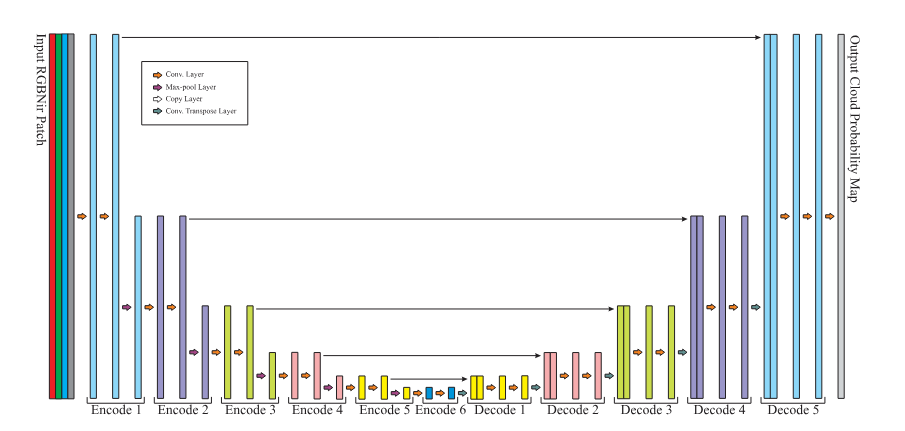
\includegraphics[width=\textwidth]{files/U-Net_cloud_detection.png}
  \caption{U-Net architecture adapted for cloud detection as used by Mohajerani et al.~\cite{mohajerani2019cloudnet}.}
  \label{fig:unet-architecture}
\end{figure}


A key innovation in U-Net is the use of residual (skip) connections \cite{he2015deepresiduallearningimage}, which dierectly link feature maps from the encoder to corresponding layers in the decoder with the same spatial size. These connections preserve fine-grained spatial details and significantly enhance segmentation quality. Moreover, they mitigate the vanishing gradient problem, facilitating the training of deeper networks and improving convergence.

\subsection{Google Coral Dev Board Mini and Edge TPU}

Running machine learning inference on embedded systems is referred to as edge inference. The Coral dev Board Mini, developed by Google, is a compact single-board computer designed for such edge AI applications. It features quad-core MediaTek 8167s System-on-a-Chip (SoC) on the Armv8-A architecture, along with a dedicated Edge TPU – a hardware accelerator optimized for executing TensorFlow Lite models using 8-bit integer operations.

The Edge TPU delivers up to 4 trillion operations per second (TOPS) of performance while consuming only around 2 watts of power, making it ideal for use in resource-constrained environments such as satellites, where energy efficiency and reliability are crucial.

To deploy a model on Edge TPU, it must meet the following requirements:
\begin{itemize}
    \item Tensor parameters quantized
    \item Tensor sizes are constant at compile-time
    \item Model parameters (such as bias tensors) are constant at compile-time
    \item Tensors are either 1-, 2-, or 3-dimensional. If a tensor has more than 3 dimensions, then only the 3 innermost dimensions may have a size greater than 1.
    \item The model uses only the operations supported by the Edge TPU (see table 1 below). \todo{CROP the table to only relevant commands and paste it}
\end{itemize}

These requirements directly affect model architecture, training strategy, and tooling. For instance, certain operations unsopported by Edge TPU must be avoided, and quantization aware training or post-training quantization must be considered early in the development process.

The following image from Coral documentation summarizes the model conversion and deployment workflow.

\begin{figure}[H]
  \centering
  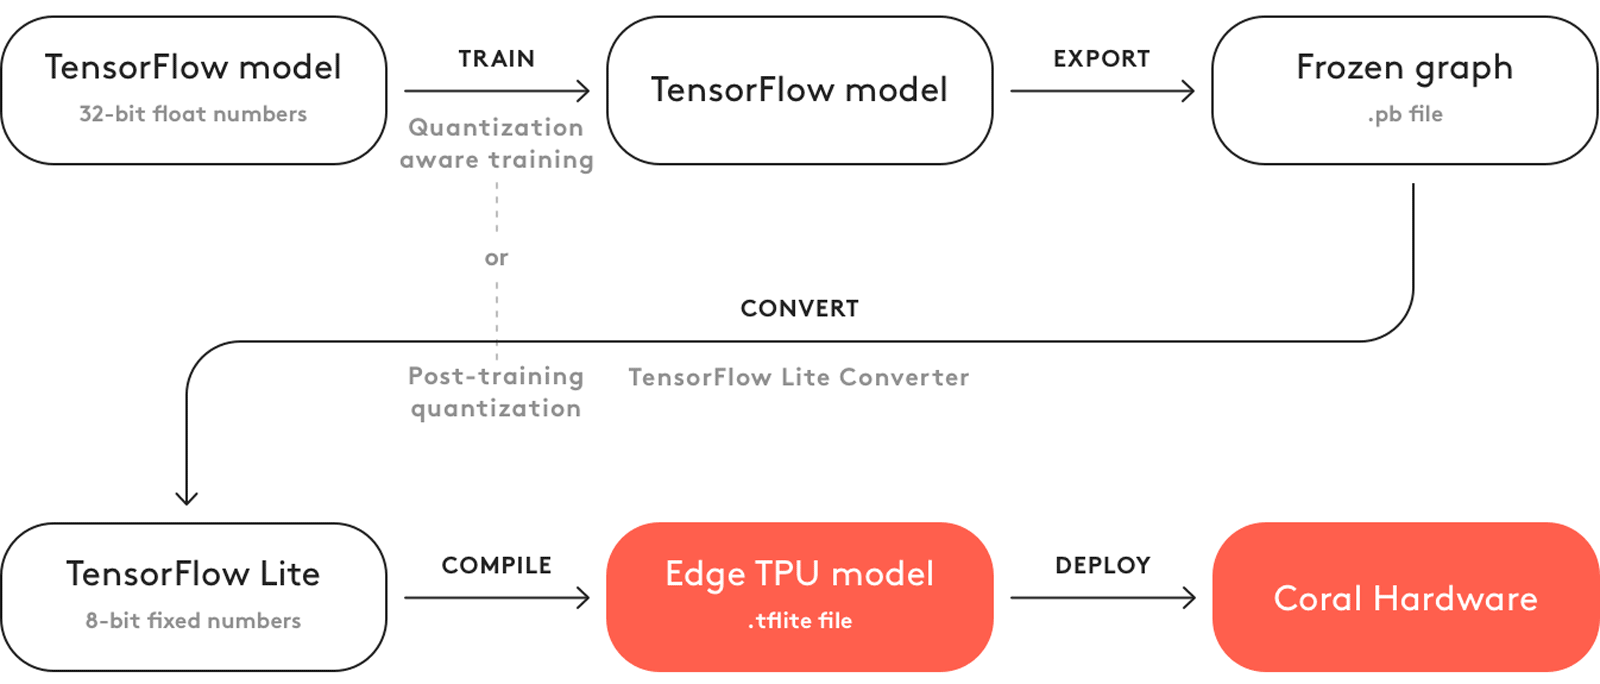
\includegraphics[width=\textwidth]{files/Edge_TPU_quantization.png}
  \caption{The basic workflow to create a model for the Edge TPU}
  \label{fig:quantization-chart}
\end{figure}

\subsection{38-Cloud Landsat 8 dataset}

Landsat 8 is an Earth observation satellite launched on February 11, 2013, providing high-resolution multispectral imagery, including visible, near infrared (NIR), and thermal infrared bands \cite{landsat8}. For cloud segmentation tasks, the red, green, blue (RGB) and NIR channels are particularly valueable due to their ability to capture both visual and athmospheric information.

This thesis utilizes a dataset consisting of 38 annotated satellite images from the Landsat 8 mission, commonly referred to as the 38-Cloud dataset \cite{38cloud}. The dataset has been introduced and adapted in the following scientific publications \cite{CloudNet2019}, \cite{CloudDet2018}. Each image contains four spectral channels (RGB and NIR), along with a manually annotated dround truth mask that labels cloud pixels at the pixel level.

The dataset is divided into a training set containing 18 scenes and a test set with the remaining 20 scenes.

}

% Optional start of thesis content
\clearpage
\setlength{\parindent}{0pt}
\setlength{\parskip}{1em}

\printbibliography
\end{document}